\lab{Barycentric Lagrange Interpolation}{Barycentric Lagrange Interpolation}
\label{lab:Barycentric}
\objective{This section explains the basic interpolation problem, and how to use Barycentric interpolation to solve the problem.}

\begin{comment}
TODO:
Point out difference between problem conditioning and numerical stability.
Using evenly spaced points as opposed to the chebyshev nodes
\end{comment}

Suppose that we have $n$ distinct points $\{x_n\}$ with associated function values $f(x_i) = y_i$. Which polynomial of degree $n$ matches the function at the specified points? This problem is known as polynomial interpolation. It is important in a variety of fields, including numerical integration(which we will cover in the next few labs).

A polynomial of degree $n$ can be written as

\[
p(x) = a_0 + a_1 x + \ldots + a_n x^n
\]
Now, by collecting our coefficients we can actually reformulate our problem as a matrix equation:
\[
\begin{pmatrix}
1 & x_1 & x_1^2 & \ldots & x_1^n \\
1 & x_2 & x_2^2 & \ldots & x_2^n \\
\vdots & \vdots & \vdots & \ddots & \vdots \\
1 & x_n & x_n^2 & \ldots & x_n^n \\
\end{pmatrix} \begin{pmatrix}
a_0 \\
a_1 \\
\vdots \\
a_n
\end{pmatrix} = \begin{pmatrix} y_1 \\ y_2 \\ \vdots \\ y_n \end{pmatrix}
\]

The matrix on the left of this equation is known as a Vandermonde matrix. It can be proven that Vandermonde matrix will have non-zero determinant if and only if  all of the $x_n$ are distinct. This implies that the equation has a unique solution, or in other words that the polynomial interpolation problem has a unique solution. The command \li{sp.vander} creates a flipped version of our Vandermonde matrix (there are several naming conventions, and \li{sp.fliplr(sp.vander())} will create the matrix we're talking about).

However, this formulation is not very useful for actually solving for the coefficients $a_i$. This is because the matrix is severely ill-conditioned.

\begin{lstlisting}
>>> import numpy as np
>>> # To work around hardware limitations we need to use floats in
>>> # our np.arange.  Otherwise, integer overflow will occur producing
>>> # incorrect results.
>>> np.linalg.cond(np.vander(np.arange(1.0,16.0)))
2.5824111670978156e+21
\end{lstlisting}

This is an astronomically large condition number for a $15 \times 15$ matrix. Even if we consider ``nicer'' interpolation points $x_n$ as in the following code, the matrix is still poorly-conditioned (we'll discuss these nicer interpolation points, known as the Chebyshev nodes, later):

\begin{lstlisting}
>>> import scipy as sp
>>> ind = np.arange(1,16)
>>> np.linalg.cond(np.vander(np.cos((2*ind-1)*np.pi/30.0)))
118998.85202836856
\end{lstlisting}

We can clearly see that the Vandermonde matrix approach is not a good approach computationally.

Instead, we take a different approach. Consider the order $n$ polynomial $L_j$ that has the properties:
\[
L_j(x_i) = \begin{cases} 0 &\mbox{ if } i \neq j\\ 1 &\mbox{ if } i =j \\ \end{cases}
\]

We already know that such a polynomial exists and is unique by the arguments above. Furthermore, we can solve our interpolation problem using the data $y_j$ through the following equation:
\[
p(x) = \sum_{j=1}^n y_j L_j(x)
\]

How do we actually calculate the $L_j$? The formula most commonly given in numerical analysis textbooks is
\[
L_j(x) = \frac{\displaystyle\prod_{k=1, k \neq j}^n (x-x_k)}{\displaystyle\prod_{k=1, k \neq j}^n (x_j-x_k)}
\]

These polynomials $(L_j)$ are known as the Lagrange basis functions. Solving the interpolation problem using these basis functions is known as Lagrange Interpolation.

\begin{problem}
Write a function that returns the Lagrange interpolant as a callable function. It should accept the $x$ and $y$ values of the desired function. Test your function on Runge's function on the interval $[-1,1]$:
\[
f(x) = \frac{1}{1+25x^2}
\]
\end{problem}

\begin{problem}
Because of the behavior of the this type of interpolation, it is highly recommended to use Chebyshev Nodes for your input $x$ values:
\[
x_i = \cos\left(\frac{(2i-1)\pi}{2n}\right), i = 1\ldots n
\]
Test the function you wrote in the previous problem using the Chebyshev nodes. How many interpolating points can your function handle before it breaks down? Test the temporal complexity of your function (You should get something like $O(n^2)$).
%the function becomes unstable around 661 points
\end{problem}

You should have noticed that the function blew up with sufficiently large $n$. This is due to numerical instability inherent to our formulation of the Lagrange basis functions. Also, the $O(n^2)$ runtime is slower than desirable.

We digress for just a moment to explain the choice of interpolation points. Why don't we select interpolation points uniformly? It actually turns out that evenly spaced interpolation points are inherently ill-conditioned. This is since a small error in a value $f_k$ near the middle of the interval of interpolation can cause large errors in the interpolant near the boundaries of the interval.

An illustration might be useful. Consider Runge's function from the previous exercise. I generated Figure \ref{Fig:Runge} using the following code:

\begin{lstlisting}
import scipy as sp
import matplotlib.pyplot as plt
ipoints = sp.linspace(-1,1,15)
runge = lambda x: 1.0/(1+25.0*x**2)
xin = sp.linspace(-1,1,1000)
plt.plot(xin,LInterp1(xin,ipoints,runge(ipoints)),'r')
plt.hold(True)
plot(xin, runge(xin))
\end{lstlisting}

As you can see in Figure \ref{Fig:Runge} even for a small number of equally spaced interpolation points the interpolant begins to diverge from the function at the edges of the interval. This is known as \emph{Runge's Phenomenon}.

\begin{figure}
\begin{center}
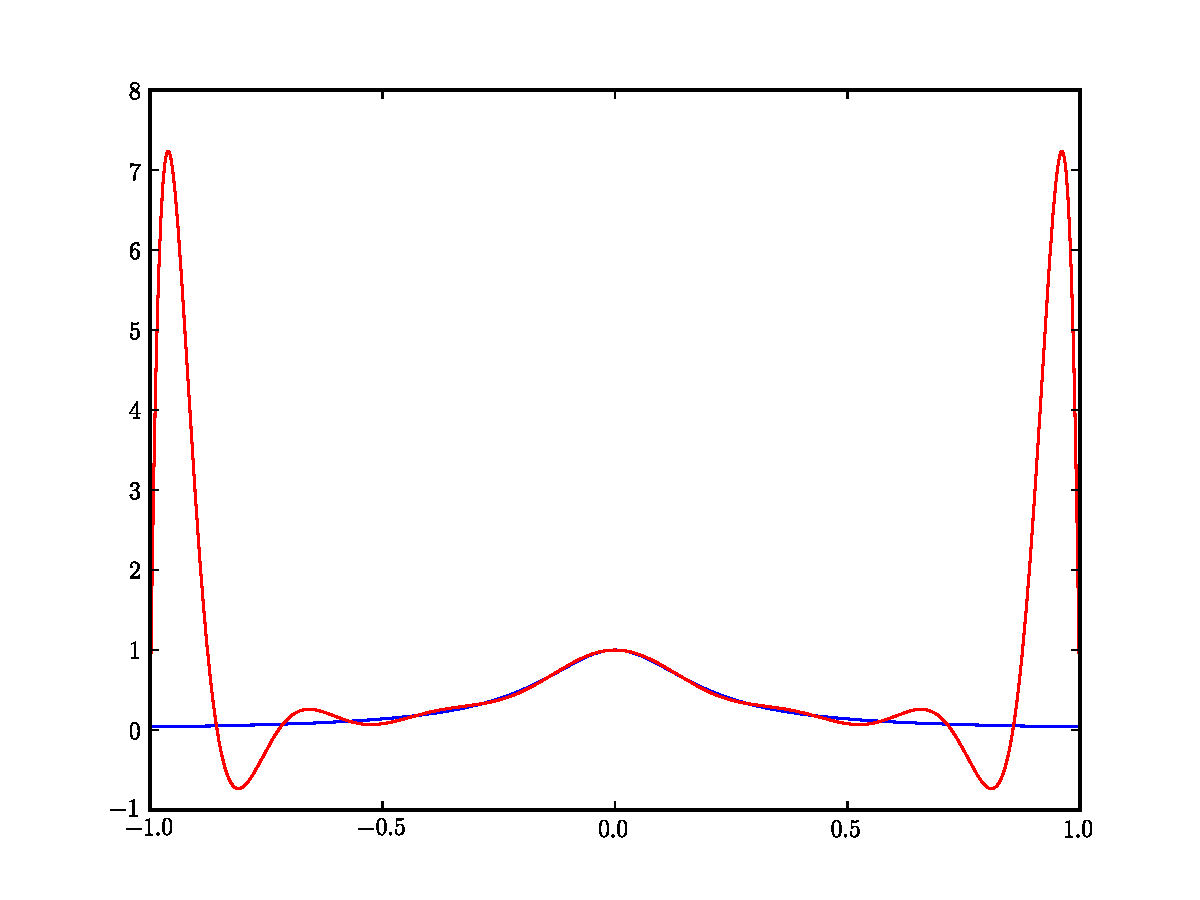
\includegraphics[scale = .5]{Runge.pdf}
\caption{An illustration of Runge's Phenomenon, using 15 interpolation points}
\label{Fig:Runge}
\end{center}
\end{figure}


To avoid this phenomenon we must select points that are distributed in a very specific way: with more points on the edge of the interval than the center. The Chebyshev Nodes are one such set of points.

It turns out that we can improve this process greatly by making a few minor modifications. We can rewrite the formulation of our basis functions as follows:
\[
L_j(x) = l(x)\frac{\frac{1}{(x-x_j)}}{\displaystyle\prod_{k=1, k \neq j}^n (x_j-x_k)}
\]

where $l(x) = \prod_{k=1}^n (x-x_k)$. This then allows us to write the interpolating polynomial in the following form:
\[
p(x) = l(x) \sum_{k=1}^n \frac{w_k y_k}{x-x_k}
\]

Where $w_k = \frac{1}{\prod_{k=1, k \neq j}^n (x_j-x_k)}$. This form requires only $O(n)$ computations, a considerable improvement. Furthermore, we note that
\[
1 = l(x) \sum_{k=1}^n \frac{w_k}{x-x_k}
\]

Which allows us to rewrite the interpolating polynomial as:

\[
p(x) = \frac{\displaystyle\sum_{k=1}^n \frac{w_k y_k}{x-x_k}}{\displaystyle\sum_{k=1}^n \frac{w_k}{x-x_k}}
\]

Rewriting the Lagrange interpolant in this form is known as \emph{Barycentric Lagrange Interpolation}. This form has the additional advantage that it is numerically stable.

We also note that this formulation makes it clear that we can ignore any factors that are common to the $w_k$ (since they will show up in both the numerator and denominator). This proves critical to the success of our formula (otherwise we will overflow the floating point arithmetic). The easiest way to combat this phenomenon is to multiply each $(x_j-x_k)$ by $C^{-1}$, where $4C$ is the width of the interval on which we are interpolating. This can be done using the following code:

\begin{lstlisting}
D = sp.max(ipoints)-sp.min(ipoints)
C = D/4.0
w = sp.zeros_like(ipoints.T)
# Calculate Barycentric Weights
shuffle = sp.random.permutation(len(ipoints)-1)
for k in range(len(ipoints)):
    test = (ipoints[k]-ipoints)/C
    test = sp.delete(test, k)
    test=test[shuffle]
    w[k] = 1.0/sp.prod(test)
\end{lstlisting}

Here we use the \li{sp.random.permutation} function so that the arithmetic doesn't overflow due to poor ordering (if we use the standard ordering we can still get overflow errors because all of the points greater (or less) than one are multiplied together at the same time).

\begin{problem}
Write a new function implementing Barycentric Lagrange Interpolation. Compare runtime with the first function you wrote. Also test how many interpolation points can be handled using this approach (this number should be in the thousands). Use Runge's function again for your tests.
\end{problem}

The Barycentric approach also has other desirable properties (such as easy addition of new points, possible pre-computation of weights etc.). It is a powerful, and yet elegant computation tool. 